\subsection{Auswertung}
Bei der Analyse des vorgegebenen Pulvers mittels Debye Scherrer Verfahren ergab sich das Diffraktogramm in Abb. ??.
\begin{figure}[H]
\centering
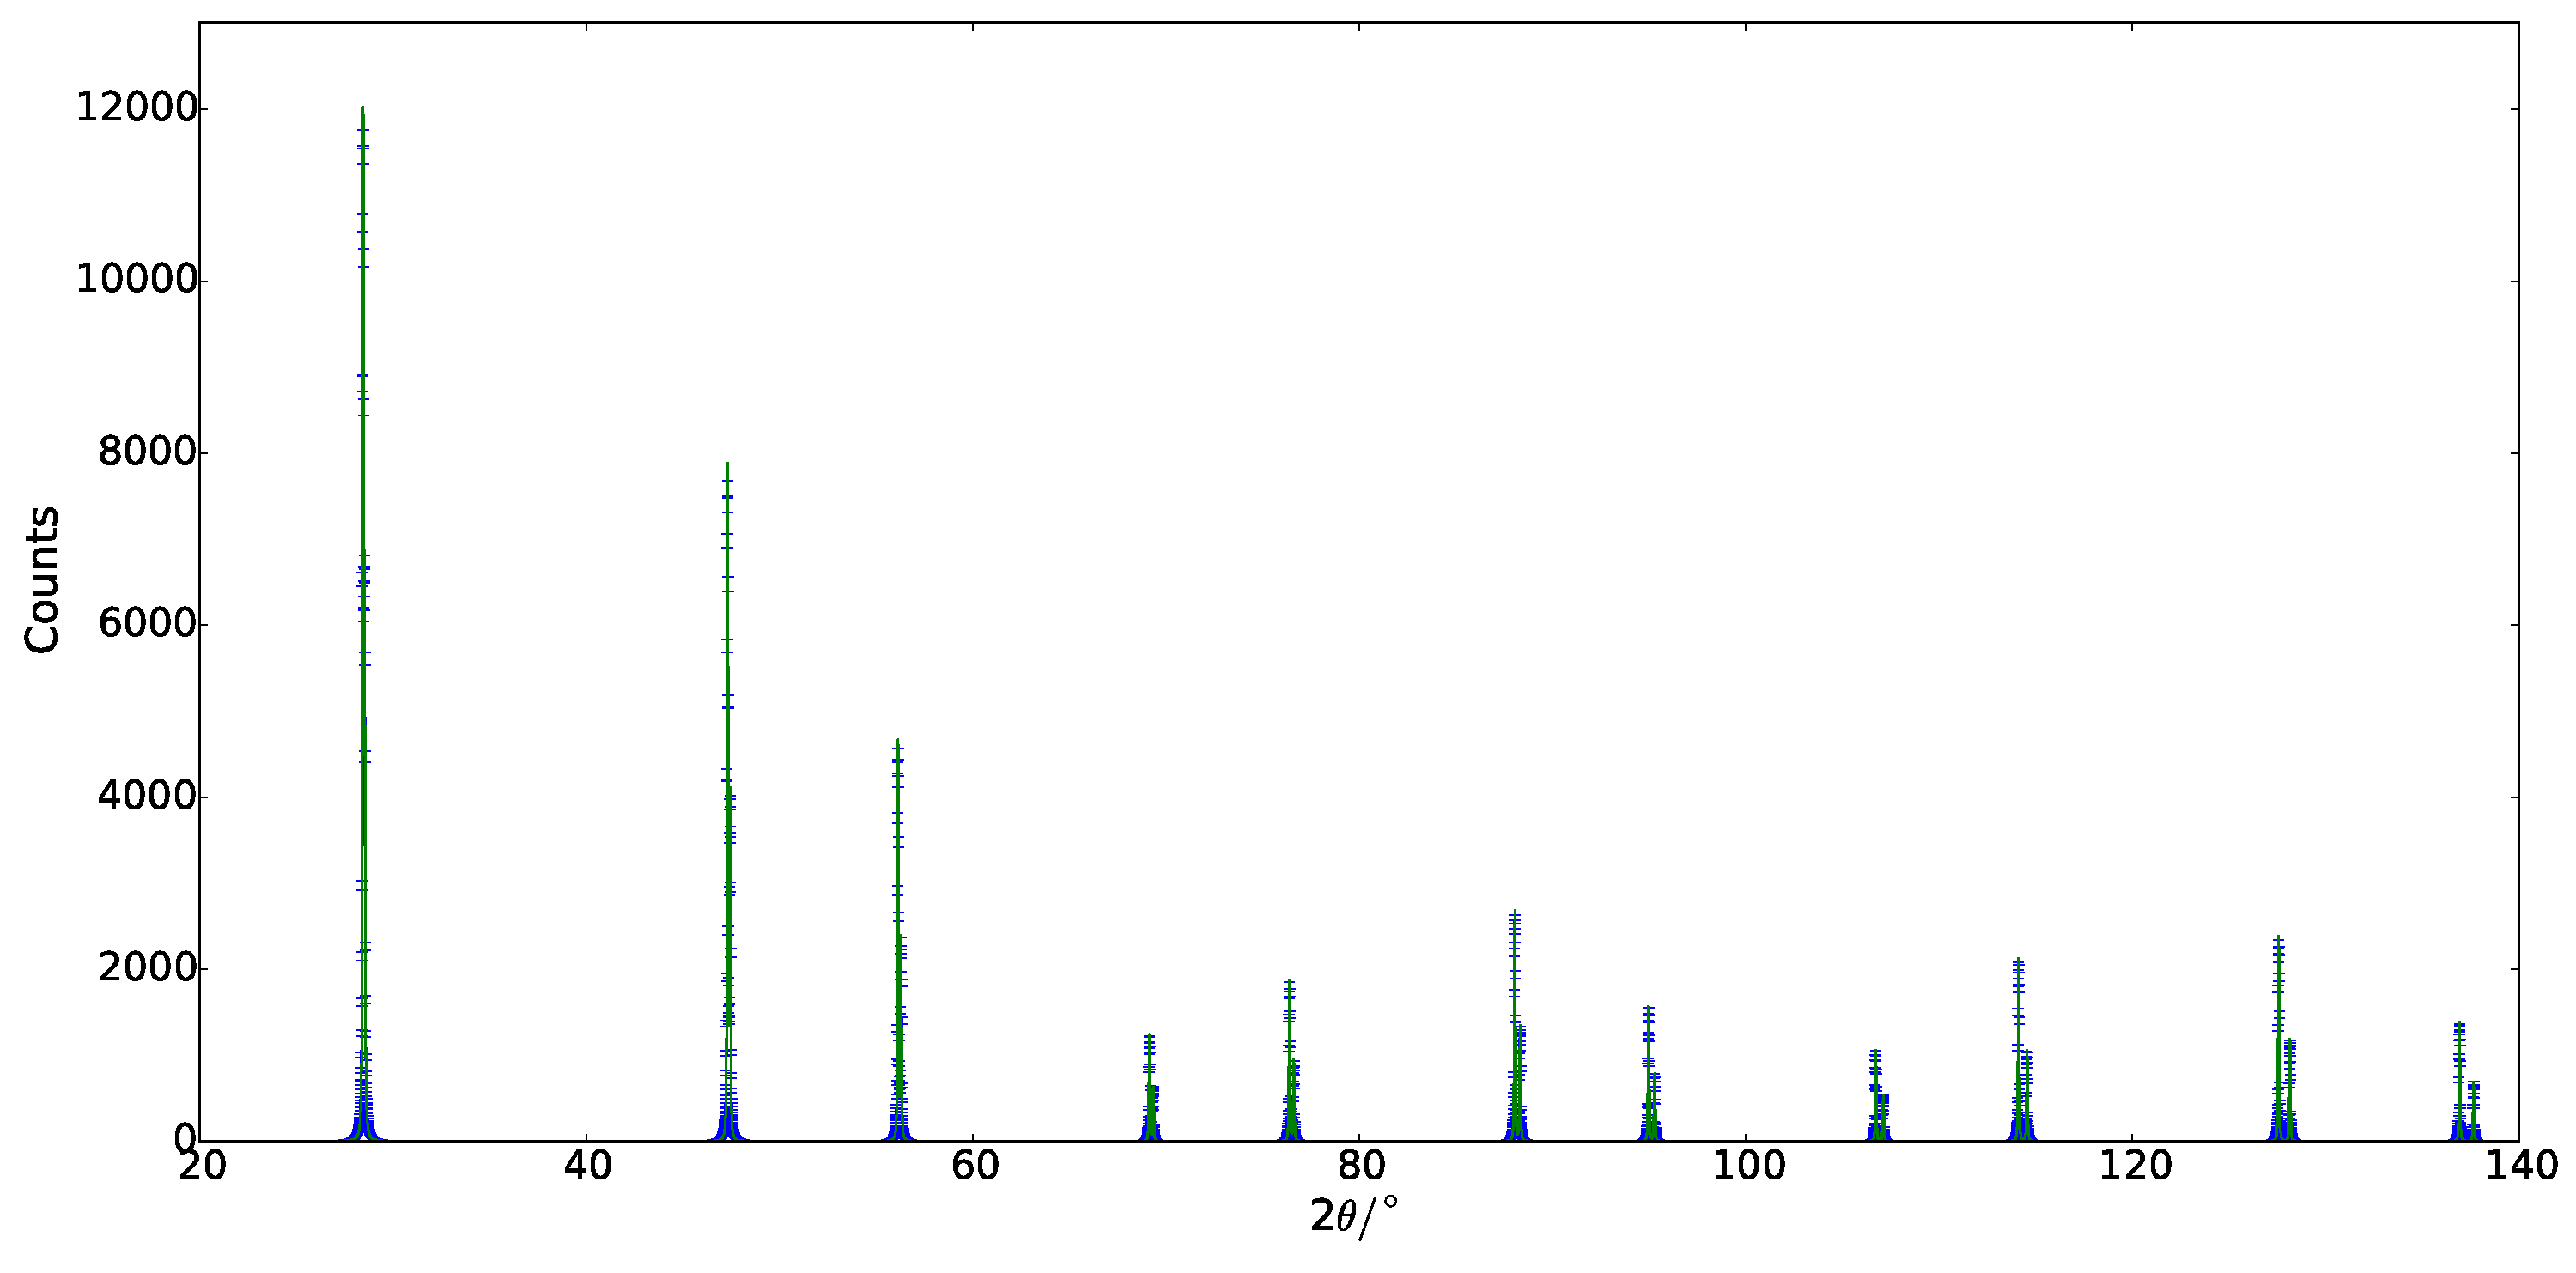
\includegraphics[angle = 90, width = 1.05\textwidth, height = 1.55\textwidth]{messung_pulver_ges}
\end{figure}
Zum Vergleich sind Diffraktogramme von Silicium und Germanium (Abb. ??) simuliert worden. Man sieht sofort, dass das Diffraktogramm von Silicium mit dem der untersuchten Probe sehr gut �bereinstimmt. Daneben stellt man einen Offset der simulierten Daten zu den gemessenen fest. Um diesen Offset zu bestimmen, wurde an alle drei Datens�tze ein Multivoigt gefittet. Die Voigtverteilung wird dabei numerisch approximiert, wobei die in Python bereits implementierte Voigt-Verteilung aus der Bibliothek "`lmfit"' verwendet wird. Der Fit an die Messdaten passt mit einem reduzierten Chiquadrat von 9,419 relativ gut, wenn man beachtet, dass auch bei kleineren Zahlraten ein Fehler von $\sqrt{N}$ verwendet wurde. Erstaunlicherweise passen die Fits, bei einem Fehler von $\sqrt{N}$, eher schlecht an die simulierten Daten. Man sieht aber, dass die Maxima trotzdem gut getroffen werden, was in diesem Versuchsteil das wichtigste Kriterium f�r die Auswertung ist. Es ergeben sich reduzierte Chiquadrate von 500 bis 20000, sodass diese Fits nicht als besonders gut betrachtet werden k�nnen. Wie die Fits in der N�he einzelner Peaks aussehen, kann im Anhang nachvollzogen werden.